\documentclass[10pt]{beamer}
\usepackage{amsmath}
\usepackage{amssymb}
\usepackage{geometry}
\usepackage{graphicx}
\usepackage{url}
\usepackage{bm}

\begin{document}

\begin{frame}
\large Lecture 14:\\ 
Simple Linear Regression\\
STAT 630, Fall 2021
\end{frame}

%-------------------------------------------
\begin{frame}{Scatterplots}
\begin{itemize}
\item A scatterplot a graphical display used to study the relationship between two variables $x$ and $y$.  
\vspace{5pt}
\item Data displayed on a scatterplot are collected in pairs:
$$(x_1, y_1), (x_2, y_2), \cdots, (x_n, y_n)$$
where $n$ denotes the total number of cases or pairs.
\vspace{5pt}
\item A scatterplot provides insight into how two variables are related. 
\end{itemize}
\end{frame}

%-------------------------------------------
\begin{frame}[fragile]{Example}
\small
\begin{verbatim}
> library(MASS)
> plot(Cars93$Weight, Cars93$MPG.highway, 
    xlab = "Weight (lbs)", ylab = "Highway MPG")
\end{verbatim}
\begin{figure}
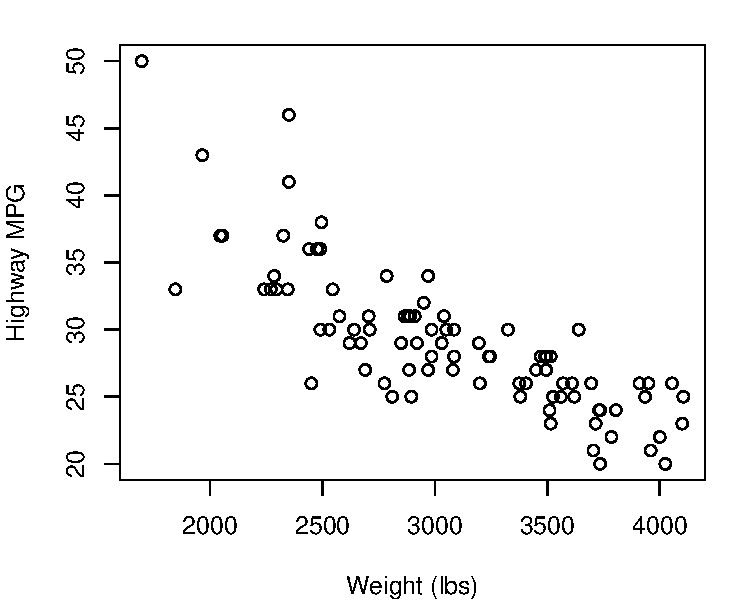
\includegraphics[scale=0.5]{figure/mpg_scatter.pdf}
\end{figure}
\end{frame}

%-------------------------------------------
\begin{frame}{Types of Relationships between Variables}
\begin{itemize}
\item Two variables are said to be \textbf{associated} if the scatterplot shows a discernible pattern or trend.
\vspace{5pt}
\item An association is \textbf{positive} if $y$ increases as $x$ increases.
\vspace{5pt}
\item An association is \textbf{negative} if $y$ decreases as $x$ increases.
\vspace{5pt}
\item An association is \textbf{linear} if the scatterplot between $x$ and $y$ has a linear trend; otherwise, the association is called \textbf{nonlinear}. 
\end{itemize}
\end{frame}

%-------------------------------------------
\begin{frame}
\centering
\begin{figure}
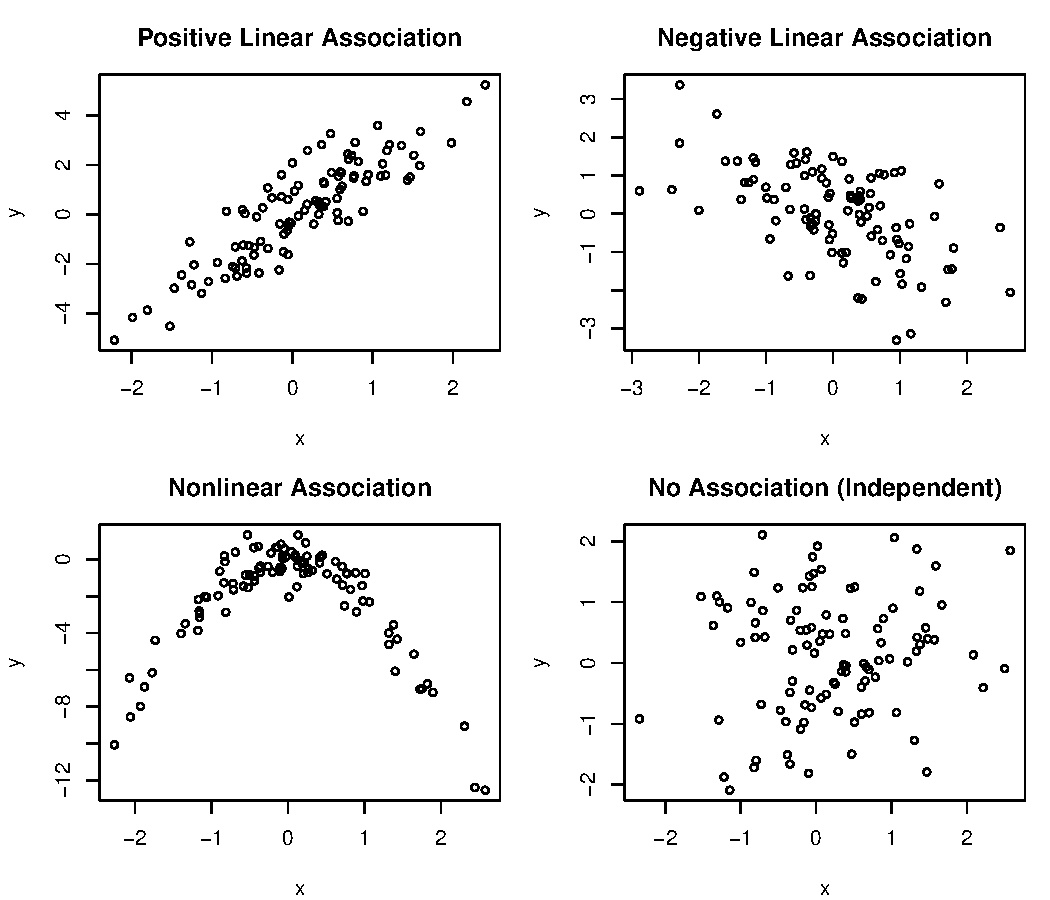
\includegraphics[scale=0.5]{figure/associations.pdf}
\end{figure}
\end{frame}

%-------------------------------------------
\begin{frame}{Correlation Coefficient}
The \textbf{correlation coefficient}, denoted by $r$, is a number between -1 and 1 that describes the strength of the linear association between two numerical variables.

\begin{align*}
r = \frac{\sum_{i=1}^n (x_i - \bar{x}) (y_i - \bar{y})}{\sqrt{\sum_{i=1}^n (x_i - \bar{x})^2} \sqrt{\sum_{i=1}^n (y_i - \bar{y})^2}} = \frac{1}{n-1} \sum_{i=1}^n \left(\frac{x_i - \bar{x}}{s_x} \right) \left( \frac{y_i - \bar{y}}{s_y} \right)
\end{align*}
\begin{itemize}
\item $\bar{x}$ and $\bar{y}$ are the sample means
\item $s_x$ and $s_y$ are the sample standard deviations
\end{itemize}
\end{frame}

%-------------------------------------------
\begin{frame}{Correlation Coefficient}
\begin{figure}
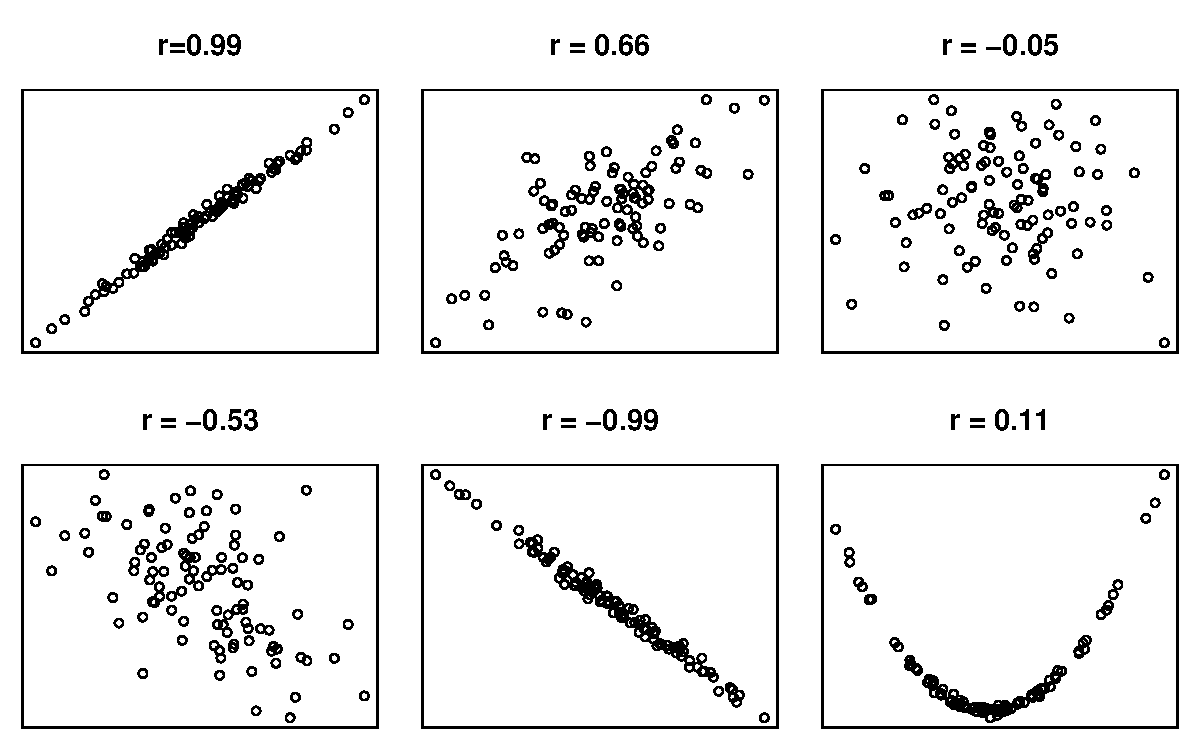
\includegraphics[scale=0.5]{figure/correlations.pdf}
\end{figure}
\end{frame}

%-------------------------------------------
\begin{frame}{Correlation Coefficient}
\begin{itemize}
\item $r \approx 1$ when there is a strong positive linear association between the variables.
\vspace{5pt}
\item $r \approx -1$ when there is a strong negative linear association between the variables.
\vspace{5pt}
\item $r \approx 0$ when there is no relationship between the variables (i.e., independent).
\vspace{5pt}
\item The correlation coefficient is only useful for evaluating the linear association between two variables.  It is not a useful measure for nonlinear relationships.
\end{itemize}
\end{frame}

%-------------------------------------------
\begin{frame}
\textbf{Simple linear regression} is a method for fitting a straight line to data that show a linear trend when displayed on a scatterplot.  It is a useful tool for making predictions for a quantitative response variable. \begin{figure}
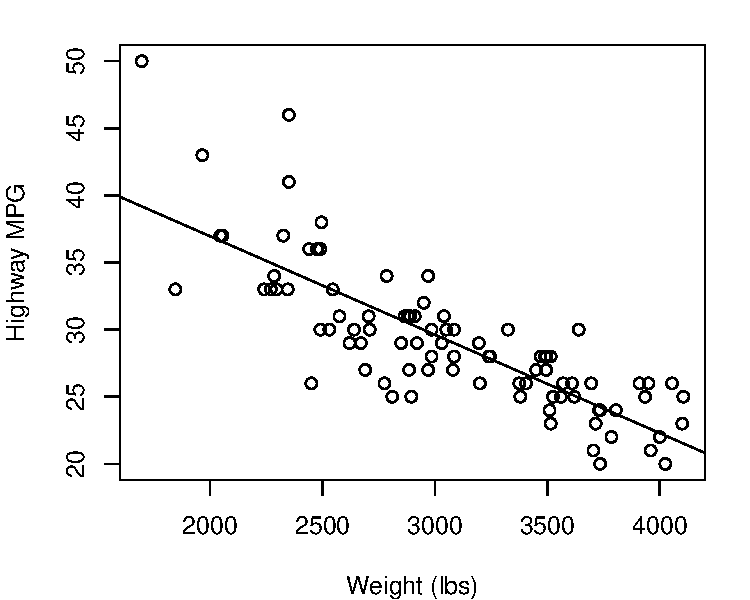
\includegraphics[scale=0.5]{figure/mpg_scatter_fit.pdf}
\end{figure}  
\end{frame}

%-------------------------------------------
\begin{frame}{Simple Linear Regression Model}
Let $\{ (x_i, y_i) : i=1, \cdots, n \}$ be a collection of $n$ data points.  A \textbf{simple linear regression model} expressing the relationship between $y_i$ and $x_i$ is given by:
$$ y_i = \beta_0 + \beta_1 x_i + \epsilon_i $$
\begin{itemize}
\item $y_i$ response variable (random)
\item $x_i$ explanatory variable (non-random)
\item $\beta_0$ intercept parameter (non-random)
\item $\beta_1$ slope parameter (non-random)
\item $\epsilon_i$ is the random error term, $\epsilon_i \sim N(0, \sigma)$\\ 
\end{itemize}
\vspace{15pt}

\footnotesize
\textbf{Remark:} $y_i$ is also sometimes called the \textbf{dependent} variable, and $x_i$ the \textbf{predictor} variable.  Notation and terminology may vary depending on the textbook and context.
\end{frame}

%-------------------------------------------
\begin{frame}{Fitted Values and Residuals}
The line that we estimate, or fit to the data in the scatterplot, is written as
$$\hat{y} = \hat{\beta}_0 + \hat{\beta}_1 x$$\\
\vspace{10pt}

The fitted (or predicted) value for the $i^{th}$ observation $(x_i, y_i)$:
$$\hat{y}_i = \hat{\beta}_0 + \hat{\beta}_1 x_i$$\\
\vspace{10pt}

The \textbf{residual} for the $i^{th}$ observation is the difference between the observed value ($y_i$) and the predicted value ($\hat{y}_i$):\\
$$\hat{e}_i = y_i - \hat{y}_i = y_i - (\hat{\beta}_0 + \hat{\beta}_1 x_i)$$
\end{frame}

\begin{frame}
\begin{figure}
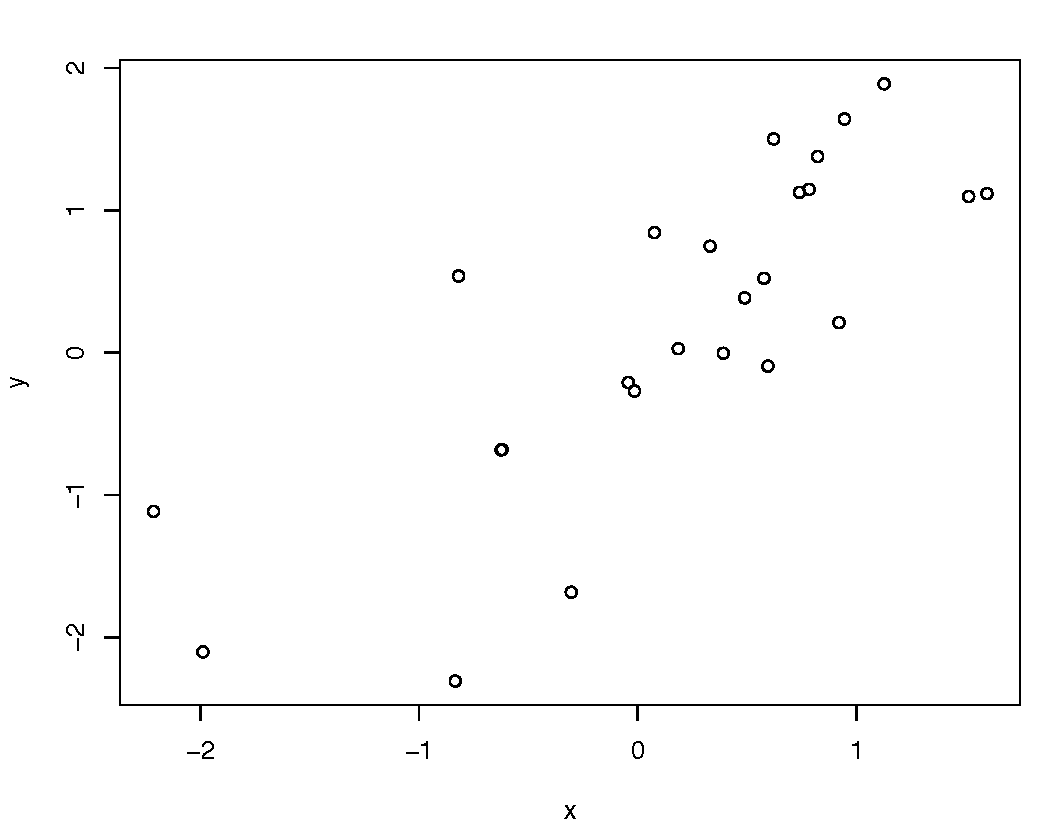
\includegraphics[scale=0.5]{figure/scatter1_2.pdf}
\end{figure}
\end{frame}

\begin{frame}
\begin{figure}
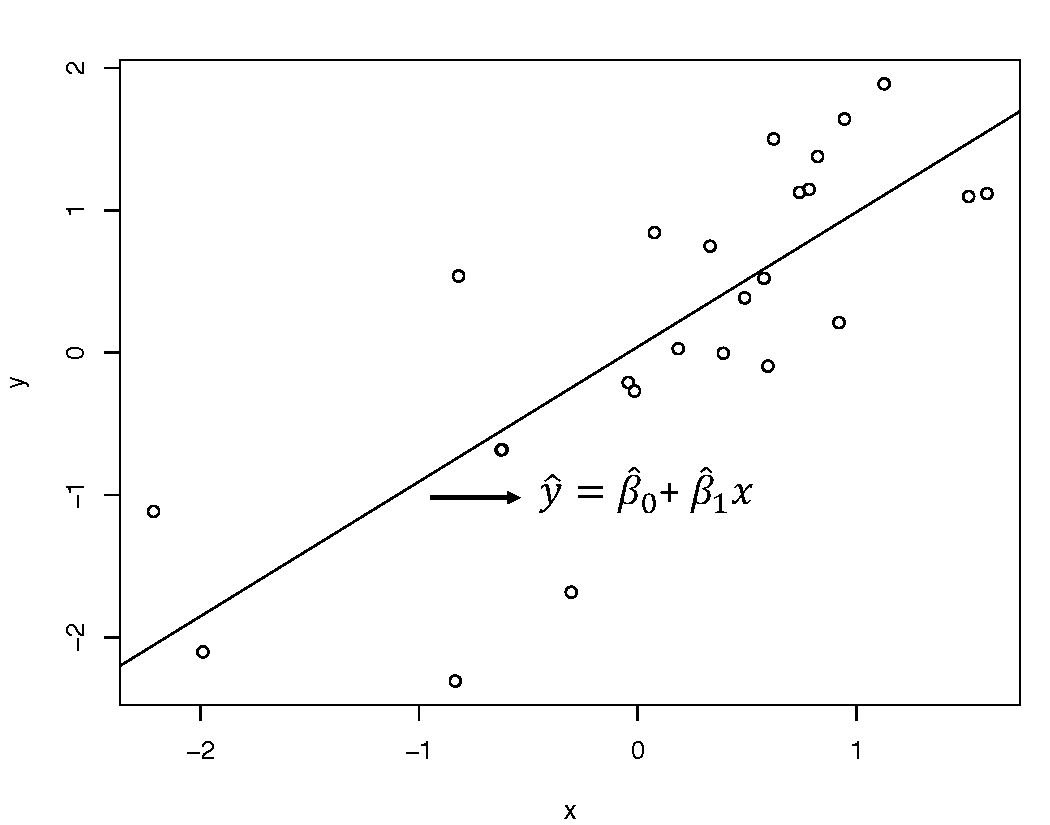
\includegraphics[scale=0.5]{figure/scatter2_2.pdf}
\end{figure}
\end{frame}

\begin{frame}
\begin{figure}
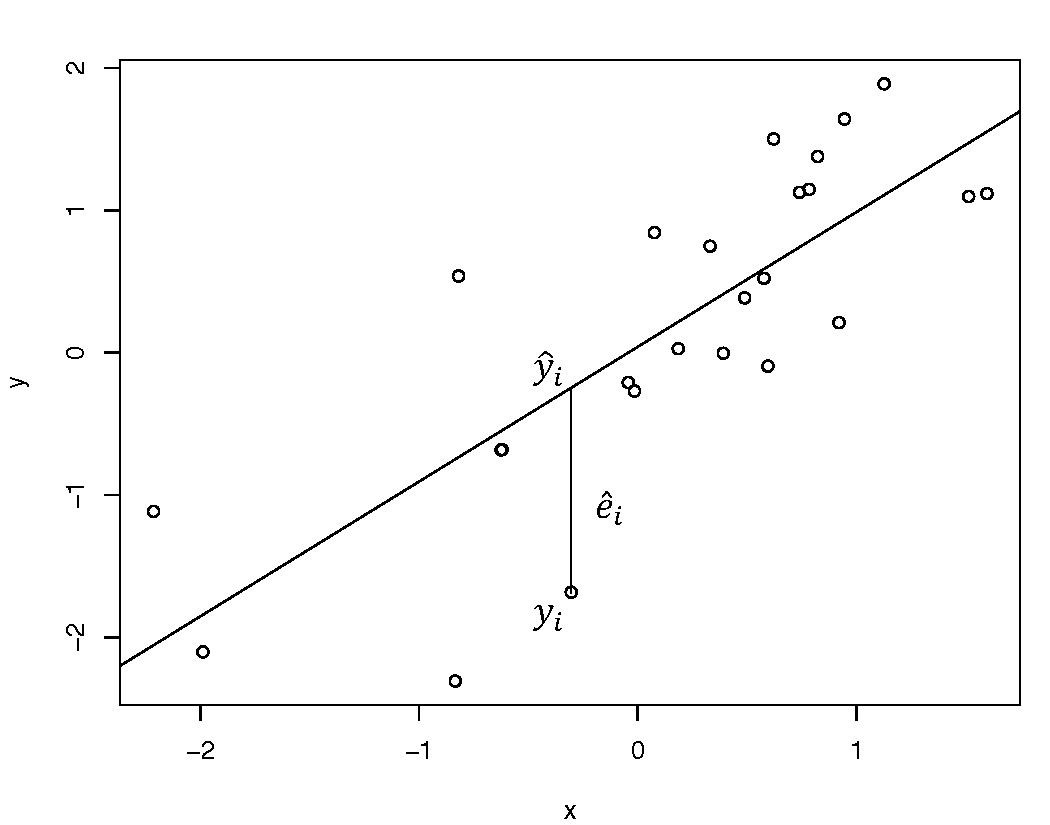
\includegraphics[scale=0.5]{figure/scatter3_2.pdf}
\end{figure}
\end{frame}

\begin{frame}
\begin{figure}
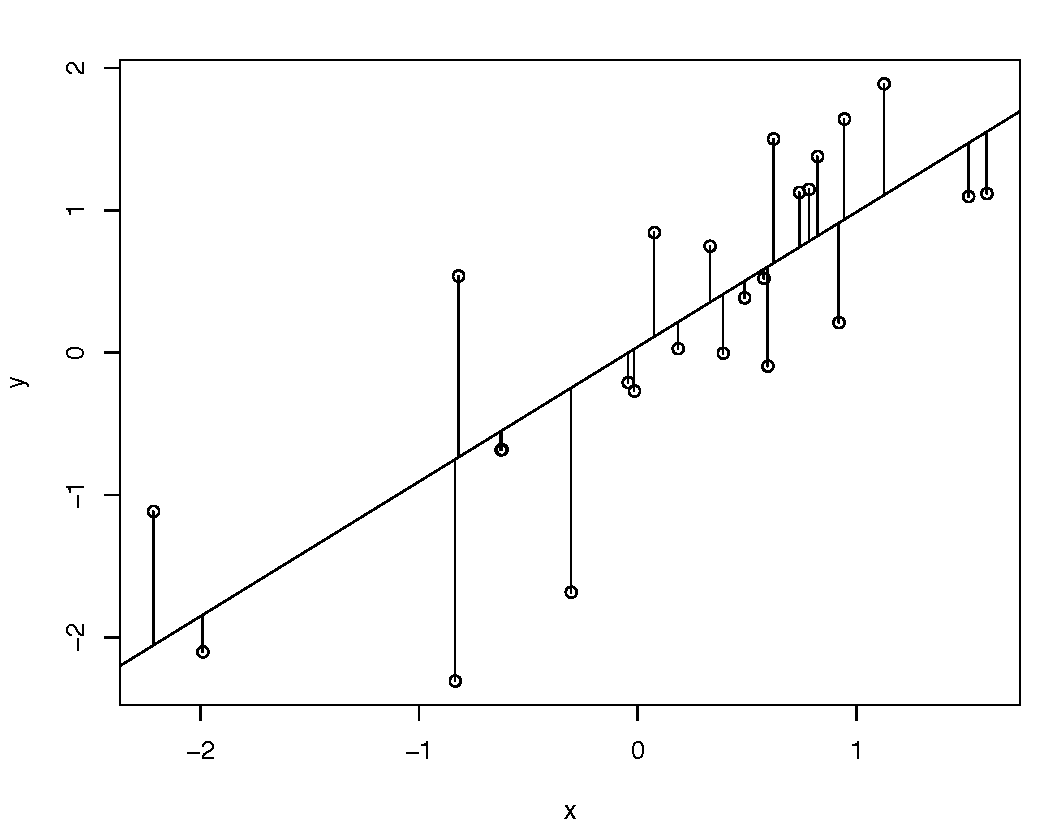
\includegraphics[scale=0.5]{figure/scatter4_2.pdf}
\end{figure}
\end{frame}

%-------------------------------------------
\begin{frame}{Sum of Squared Residuals}
\begin{itemize}
\item Intuitively, a line that fits the data well has small residuals.
\vspace{5pt}
\item The \textbf{least squares line} minimizes the \textbf{sum of squared residuals}:
$$RSS = \sum_{i=1}^n \hat{e}_i^2 = \sum_{i=1}^n (y_i - \hat{\beta}_0 - \hat{\beta}_1 x_i)^2$$
\vspace{5pt}
\item That is, out of all possible lines we could draw on the scatterplot, the least squares line is the ``best fit" since it has the smallest sum of squared residuals.
\end{itemize}
\end{frame}

%-------------------------------------------
\begin{frame}{Least Squares Estimation}
Formally, the estimates $\hat{\beta}_0$ and $\hat{\beta}_1$ of the intercept and slope are found by using calculus to minimize the sum of squared residuals:
\begin{align*}
RSS = \sum_{i=1}^n \hat{e}_i^2 = \sum_{i=1}^n (y_i - \hat{\beta}_0 - \hat{\beta}_1 x_i)^2
\end{align*}

To minimize set the partial derivatives equal to zero:\\
\begin{align*}
\frac{\partial RSS}{\partial \hat{\beta}_0} &= -2 \sum_{i=1}^n (y_i - \hat{\beta}_0 - \hat{\beta}_1 x_i) = 0\\
\frac{\partial RSS}{\partial \hat{\beta}_1} &= -2 \sum_{i=1}^n x_i (y_i - \hat{\beta}_0 - \hat{\beta}_1 x_i) = 0
\end{align*}
\end{frame}

%-------------------------------------------
\begin{frame}
\end{frame}

%-------------------------------------------
\begin{frame}{Least Squares Estimation}
Using some algebraic manipulation we can solve these two equations to obtain the least squares estimates of the intercept and slope:
\begin{align*}
\hat{\beta}_0 &= \bar{y} - \hat{\beta}_1 \bar{x}\\
\hat{\beta}_1 &= \frac{\sum_{i=1}^n (x_i - \bar{x})(y_i - \bar{y})}{\sum_{i=1}^n (x_i - \bar{x})^2} = r \frac{s_y}{s_x}
\end{align*}
Note that the equation for the intercept guarantees the least squares line passes through $(\bar{x}, \bar{y})$.
\end{frame}

%------------------------------------------------------
\begin{frame}{Interpretation}
\vspace{-2cm}
\begin{itemize}
\item \textbf{Slope}: an increase in the explanatory variable ($x$) by one unit is associated with a change of $\hat{\beta}_1$ in the predicted response ($\hat{y}$).
\vspace{10pt}
\item \textbf{Intercept}: the prediction for the response variable ($\hat{y}$) when the value for the explanatory variable is zero ($x=0$).  It may not make sense to try to interpret the intercept depending on the application.\\    
\end{itemize}
\end{frame}

\begin{frame}{Coefficient of Determination}
The \textbf{coefficient of determination} ($R^2$) is a measure of how well the linear regression model fits the data.
\begin{align*}
R^2 = \frac{TSS - RSS}{TSS} = 1 - \frac{RSS}{TSS}
\end{align*}
\vspace{10pt}
\begin{itemize}
\item $TSS=\sum_{i=1}^n (y_i - \bar{y})^2$ is the total sum of squares (total variability in the response variable) 
\vspace{5pt}
\item $RSS=\sum_{i=1}^n (y_i - \hat{y}_i)^2$ is the residual sum of squares (unexplained variability)
\end{itemize}
\end{frame}

\begin{frame}{Coefficient of Determination}
\begin{itemize}
\item $R^2$ can be interpreted as the proportion of variability in the response variable $y$ that is explained by $x$.
\vspace{5pt}
\item $0 \leq R^2 \leq 1$; the closer $R^2$ is to 1, the better the linear regression model fits the data.
\vspace{5pt}
\item $R^2$ can be computed as the correlation coefficient $r$ squared.
\vspace{5pt}
\item $R^2$ is arguably one of the most commonly misused statistics.  Always look at a scatterplot of your data first, and check whether fitting a line makes sense and for any outliers.
\end{itemize}
\end{frame}

% Next time
% Inference 


\end{document}